\let\negmedspace\undefined
\let\negthickspace\undefined
\documentclass[journal]{IEEEtran}
\usepackage[a5paper, margin=10mm, onecolumn]{geometry}
\usepackage{tfrupee} 
\setlength{\headheight}{1cm} 
\setlength{\headsep}{0mm}     

\usepackage{gvv-book}
\usepackage{gvv}
\usepackage{cite}
\usepackage{amsmath,amssymb,amsfonts,amsthm}
\usepackage{algorithmic}
\usepackage{graphicx}
\usepackage{textcomp}
\usepackage{xcolor}
\usepackage{txfonts}
\usepackage{listings}
\usepackage{enumitem}
\usepackage{mathtools}
\usepackage{gensymb}
\usepackage{comment}
\usepackage[breaklinks=true]{hyperref}
\usepackage{tkz-euclide} 
\usepackage{listings}
\def\inputGnumericTable{}                                 
\usepackage[latin1]{inputenc}                                
\usepackage{color}                                            
\usepackage{array}                                            
\usepackage{longtable}                                       
\usepackage{calc}                                             
\usepackage{multirow}                                         
\usepackage{hhline}                                           
\usepackage{ifthen}                                           
\usepackage{lscape}
\usepackage{circuitikz}
\tikzstyle{block} = [rectangle, draw, fill=blue!20, 
    text width=4em, text centered, rounded corners, minimum height=3em]
\tikzstyle{sum} = [draw, fill=blue!10, circle, minimum size=1cm, node distance=1.5cm]
\tikzstyle{input} = [coordinate]
\tikzstyle{output} = [coordinate]
\renewcommand{\thefigure}{\theenumi}
\renewcommand{\thetable}{\theenumi}
\setlength{\intextsep}{10pt} % Space between text and floats
\numberwithin{equation}{enumi}
\numberwithin{figure}{enumi}
\renewcommand{\thetable}{\theenumi}

\begin{document}

\bibliographystyle{IEEEtran}
\vspace{3cm}

\title{1.9.21}
\author{EE25BTECH11032 - Kartik Lahoti}
\maketitle

\subsection*{Question: } 
Given vertices of a parallelogram $\vec{A} \brak{-2,1} , \vec{B} \brak{a,0} , \vec{C} \brak{4,b}, \text{ and } \vec{D} \brak{1,2}$. Find the values of $a \text{ and } b $. Hence, find the lengths of its sides. \\
\solution \\ 

\subsubsection*{Given }
A parallelogram $ABCD$ with , 
\begin{align}
    \vec{A} = \myvec{-2\\1} , \vec{B} = \myvec{a\\0} , \vec{C} = \myvec{4\\b} , \vec{D} = \myvec{1\\2}     
\end{align}

\underline{\textbf{Theory :}} \\

In a Parallelogram $PQRS$ the opposite side are parallel and equal , i.e. $PQ \parallel RS $ and $PQ = RS $ and similarly  $QR \parallel  PS $ and $ QR = PS $

$\therefore$ \text{we can say, } \begin{align}\vec{AB} = \vec{DC}\end{align}

Calculating $\vec{AB}$ , 

\begin{align}
    \vec{AB} = \vec{B} - \vec{A}
\end{align}

\begin{align}
    \vec{AB} &= \myvec{a\\0} - \myvec{-2\\1} = \myvec{a+2\\-1}
\end{align}

Similarly, 
\begin{align}
    \vec{DC} &= \myvec{3\\b-2}
\end{align}

From Eqn (0.2) we get : 
\begin{align}
    \myvec{a+2\\-1} = \myvec{3\\b-2} \\
\end{align}
\begin{align}
    \implies a = 1 \text{ and }  b = 1
 \end{align}

$\therefore a = 1$ and $ b = 1 $ 

Calculating the side lengths , 

\begin{align}
    \because \vec{A} - \vec{B} = \myvec{-3\\1} , \\
    (\vec{A} - \vec{B})^\top (\vec{A} - \vec{B}) &=  10
\end{align}
Thus, the desired length $\vec{AB}$ is 
\begin{align}
		d_1=\norm{\vec{A}-\vec{B}} =\sqrt{10}
\end{align}
Similarly, 
\begin{align}
    \because \vec{B} - \vec{C} = \myvec{-3\\-1} , \\
    (\vec{B} - \vec{C})^\top (\vec{B} - \vec{C}) &=  10
\end{align}
Thus, the desired length $\vec{BC}$ is 
\begin{align}
		d_2=\norm{\vec{B}-\vec{C}} =\sqrt{10}
\end{align}

\textbf{Hence: } The length of the sides of the parallelogram is $ \sqrt{10} $

\begin{figure}[H]
    \centering
    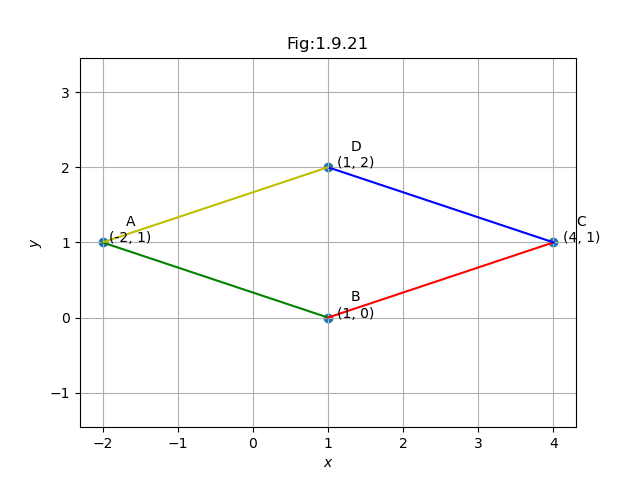
\includegraphics[width=1.0\columnwidth]{figs/p_gram1.png}
    \caption*{}
    \label{fig:}
\end{figure}

\end{document}
